
The simplest thing to say about nonlinear equations is that they change the functional form of the residual, compared to the linear case.  For a linear system the residual $\br$ is a certain function of the unknowns $\bu$, namely $\br = \bF(\bu) = \bb - A \bu$.  Now we consider cases in which $\bF$ is a higher-order polynomial, a transcendental function, or some more general function.

Suppose for now that $\bF : \RR^N \to \RR^N$ is differentiable.  The input $\bx$ and output $\bF(\bx)$ are column vectors,\sidenote{Our name change $\bu\to\bx$ comes from now thinking more geometrically about the location of $\bx$.} so in that sense $\bF$ acts like square-matrix multiplication $\bx\mapsto A\bx$.  Just as a linear solver like GMRES (Chapter \ref{chap:ls}) reduces the linear residual $\br_k=\bb - A \bu_k$ to zero by generating a sequence $\bu_k$, for nonlinear $\bF$ we want to solve
\begin{equation}
   \bF(\bx) = 0   \label{eq:nl:equation}
\end{equation}
by iteration, generating approximations $\bx_k$ so that $\bF(\bx_k)$ goes to zero.

Newton's method linearizes \eqref{eq:nl:equation} around the most recent iterate $\bx_k$ and then ``moves'' to the location $\bx_{k+1}$ which solves the linear problem.  The new location is, we hope, closer to the solution.  Each iteration requires solving a linear system, and we already have \PETSc technology for that.  However, the cost of performing the linearization must be taken into account, choosing a smart distance to move will require additional choices, and all existing choices regarding the linear solver---especially preconditioning---remain active.  Solving a nonlinear problem generally requires all the tools for linear systems considered in Chapter \ref{chap:ls}, and more.

Large systems of nonlinear equations often arise in applications from PDE-type physical models with nonlinearities.  However, the current Chapter is largely about finite-dimensional systems of nonlinear equations \eqref{eq:nl:equation} as problems of their own.  Late in this Chapter we do give an example of a discretized one-dimensional nonlinear PDE.


\section{Newton's method}

Suppose $\bx_k\in\RR^N$ is an approximation, whether good or bad, to the solution of \eqref{eq:nl:equation}.  If we have already determined a \emph{step} $\bs\in\RR^N$ away from this current iterate $\bx_k$ then $\bx_{k+1} = \bx_k + \bs$ will be the next iterate.  Because $\bF$ is differentiable, by definition
\begin{equation}
    \bF(\bx_{k+1}) = \bF(\bx_k) + J_\bF(\bx_k) \bs + o(\|\bs\|)  \label{eq:nl:expandF}
\end{equation}
for some square matrix
\begin{equation}
J_\bF(\bx_k) = \begin{bmatrix}
    \frac{\partial F_0}{\partial x_0} & \dots & \frac{\partial F_0}{\partial x_{N-1}} \\
    \vdots & \ddots & \vdots \\
    \frac{\partial F_{N-1}}{\partial x_0} & \dots & \frac{\partial F_{N-1}}{\partial x_{N-1}}  \end{bmatrix}  \label{eq:nl:jacdefn}
\end{equation}
and some quantity $o(\|\bs\|)$ that goes to zero as the \emph{step length} $\|\bs\|$ goes to zero.  The matrix $J = J_\bF(\bx_k)$ is called the \emph{Jacobian} of $\bF$ at $\bx_k$; we also call the function $\bx \mapsto J_\bF(\bx)$ the Jacobian.

Each iteration of Newton's method approximately solves \eqref{eq:nl:equation} by truncating \eqref{eq:nl:expandF}---removing ``$+o(\|\bs\|)$''---and seeking $\bs$ so that the updated value $\bF(\bx_{k+1})$ would be zero if the truncated equation were true.  That is, each Newton step computes $\bs$ by the linear equation
\begin{equation}
    0 = \bF(\bx_k) + J_\bF(\bx_k) \bs.
\end{equation}
Writing the linear system in form ``$A\bu=\bb$,'' we see that an iteration of Newton's method requires solving a linear system and then doing a vector addition:
\refstepcounter{equation}\label{eq:nl:newton}  % \eqref{eq:nl:newton} for both eqns
\begin{align}
    J_\bF(\bx_k) \bs &= - \bF(\bx_k)  \label{eq:nl:newton:eq} \tag{\theequation a} \\
    \bx_{k+1} &= \bx_k + \bs  \label{eq:nl:newton:update} \tag{\theequation b}
\end{align}
This is Newton's method.  It is fairly simple in theory.

Actual practice for Newton's method is also not that complicated with \PETSc in hand, because it has a mature implementation of this core technology.  In fact, despite the reputation of Newton iteration as fragile or scary, it works just fine on many nonlinear systems once one adds some protections.  Primarily, a line search will, as needed, move a shorter distance to the new iterate than stated in \eqref{eq:nl:newton:update}; see page \pageref{sec:linesearch}.

Finite-dimensional nonlinear systems \eqref{eq:nl:equation} can be visualized as the problem of finding the intersections of curves, surfaces, or hypersurfaces, depending on dimension.  A small example gives us a start on the details.

\clearpage
\noindent\hrulefill
\begin{example}  Given parameter $b > 1$, the nonlinear equations
    $$y = \frac{1}{b} e^{bx}, \qquad x^2+y^2 = 1,$$
form intersecting curves in the plane.  The curves intersect twice, as shown in Figure \ref{fig:expcirclebasic}.  These equations are put in standard form \eqref{eq:nl:equation} by writing

\begin{marginfigure}
\includegraphics[width=1.2\textwidth]{figs/expcirclebasic}

\medskip
\caption{Newton iterates $\bx_k$ approach a solution of $\bF(\bx)=0$ for $\bF$ in \eqref{eq:nl:expcircleF} and $b=2$.}
\label{fig:expcirclebasic}
\end{marginfigure}

\begin{equation}
\label{eq:nl:expcircleF}
\bF(\bx) = \begin{bmatrix}
           \frac{1}{b} e^{b x_0} - x_1 \\
           x_0^2 + x_1^2 - 1
           \end{bmatrix}
\end{equation}
for $\bx\in \RR^2$ a column vector: $\bx = [x_0 \,\,\, x_1]^\top$.  Thus
\begin{equation}
\label{eq:nl:ecjacobian}
J_\bF(\bx) = \begin{bmatrix}
    e^{b x_0} & & -1 \\
    2 x_0   & & 2 x_1 \end{bmatrix}
\end{equation}
As also shown in Figure \ref{fig:expcirclebasic}, for $b=2$, if we start the Newton iteration with $\bx_0 = [1 \,\, 1]^\top$ then the sequence of iterates from \eqref{eq:nl:newton} is
    $$\twovect{\bx}{0}{1}{1}, \quad \twovect{\bx}{1}{0.619203}{0.880797}, \quad \twovect{\bx}{2}{0.394157}{0.948623}, \quad \dots$$
\noindent\hrulefill
%  FROM $ for N in 0 1 2; do ./expcircle -snes_fd -snes_max_it $N; done
\end{example}


\section{Using \pSNES with call-backs} \label{sec:usingsnes}

We will compute the Newton iterates in the example above by using a nonlinear solver object of type \pSNES\sidenote{SNES stands for ``scalable nonlinear equation solver.''} from \PETSc.  Note \pSNES has the usual \texttt{Create/SetFromOptions/Destroy} sequence.  Our code provides a function $\bF$ which is a ``call-back'' in the sense that we supply it to the \pSNES, which then calls it with argument $\bx$ when it needs $\bF(\bx)$ during the Newton iteration.

Later we will also provide the \pSNES with a function which computes the Jacobian function $J_\bF$.  However, the Jacobian can be approximated by repeated $\bF$ evaluations because a derivative can also be approximated by finite differences.  Thus our first code avoids such a Jacobian ``call-back.''

The whole of \texttt{expcircle.c}, to solve the above Example, is in Code \ref{code:expcircle}.  The \texttt{main()} method starts by allocating \pVec \texttt{x} of fixed dimension 2 which will hold the initial iterate $\bx_0$.  (Once the Newton iteration is ended it holds the converged estimate of the solution.)  Because both components of $\bx_0$ are $1$, it is initialized using \texttt{VecSet()}.  Next a duplicate \pVec \texttt{r} is created because the \pSNES needs it as space to store the (nonlinear) residual.

Then the \pSNES is created and configured.  Formula \eqref{eq:nl:expcircleF} is in method \texttt{FormFunction()}, which is supplied to the \pSNES object using \texttt{SNESSetFunction()}.  We call \texttt{SNESSetFromOptions()} because it gives us run-time control on how the Jacobian is calculated\sidenote{Options \texttt{-snes\_fd} and \texttt{-snes\_mf} are allowed; see Table \ref{tab:snesjacobianoptions:needed} below.} and on how the length of the step $\bs$ is determined.\sidenote{Through \texttt{-snes\_linesearch\_type} and related options; see page \pageref{sec:linesearch}.}  Then \eqref{eq:nl:equation} is solved by a call to \texttt{SNESSolve()}.  Finally the new values in \texttt{x}, presumably the converged solution, are printed at the command line using \texttt{VecView()} with a \texttt{STDOUT} viewer.

\vfill
\cinput{expcircle.c}{\CODELOC}{A first \pSNES-using code.  Solves nonlinear system \eqref{eq:nl:equation} with $\bF$ given in \eqref{eq:nl:expcircleF}.}{//START}{//END}{code:expcircle}

In order to match the calling sequence of \texttt{SNESSetFunction()}, \texttt{FormFunction()} must have a particular ``signature'' as a C function:
\begin{code}
PetscErrorCode (*f)(SNES,Vec,Vec,void*)
\end{code}
In particular, \texttt{FormFunction()} takes the input $\bx$ as the first \pVec and it generates output $\bF(\bx)$ as the second \pVec.\sidenote{For the second \pVec argument, note that a \pVec is in reality a \emph{pointer}, so passing a \pVec by value allows it to be modified.}

In other examples there may be additional information, such as parameters, passed to \texttt{FormFunction()} in a ``user context.''  This is why there is a fourth pointer argument ``\texttt{void*}'' to \texttt{FormFunction()}.  We will show how to pass parameters in the next code.

Looking inside \texttt{FormFunction()} in Code \ref{code:expcircle}, we see a new method for extracting values from, and setting values in, a \pVec.  Previously we have used \texttt{VecSetValues()} to set values at given indices (Chapter \ref{chap:ls}), or we have used a \pDMDA structured grid method of access (Chapter \ref{chap:st}).  Here we access the C array underlying the \pVec.  Because we only need to read entries of input \pVec \texttt{x}, we use the read-only array access method \texttt{VecGetArrayRead()} which supplies us with a read-only pointer ``\texttt{const double *ax}.''\sidenote{Because of the \texttt{const} qualifier, the C compiler can stop us from altering \texttt{ax[0]}, for example.  Try it!}  Since we are setting entries of \pVec \texttt{F}, we do nearly the same for it but we use an unrestricted pointer ``\texttt{double *aF}'' and method \texttt{VecGetArray()}.

Note that to avoid conflicts with other methods which might want to read or write to the same memory, calls to \texttt{VecGetArray()} and \texttt{VecGetArrayRead()} are matched by \texttt{VecRestoreArray()} and \texttt{VecRestoreArrayRead()}.  These methods ``free-up''  the \pVecs, but they do not deallocate anything.\sidenote{\texttt{VecDestroy()} does that.}  In general:
\begin{quote}
\emph{Each \emph{\texttt{VecGetArray()}}-type call should be matched by the corresponding \emph{\texttt{VecRestoreArray()}} call once you are done with the array.}
\end{quote}

The actual content of \texttt{FormFunction()} is to implement formulas \eqref{eq:nl:expcircleF}.  \texttt{PetscExpReal()}, which computes the exponential function $e^x$, is just an alias for \texttt{exp()} from the standard library (i.e.~\texttt{math.h}).  Use of such \PETSc library functions means that the \PETSc configuration can link to consistent libraries just by including \texttt{petsc.h}.

It is time to run this example with \texttt{-snes\_monitor}, so as to count the iterations and show the residual norm $\|\bF(\bx_k)\|_2$:
\begin{cline}
$ cd c/ch4/
$ make expcircle
...
$ ./expcircle -snes_fd -snes_monitor
  0 SNES Function norm 2.874105323289e+00 
  1 SNES Function norm 8.591393113962e-01 
  2 SNES Function norm 1.609958353862e-01 
  3 SNES Function norm 1.106891696425e-02 
  4 SNES Function norm 6.618141730691e-05 
  5 SNES Function norm 2.420782802130e-09 
Vec Object: 1 MPI processes
  type: seq
0.319632
0.947542
\end{cline}
%$
Thus after 5 iterations the Newton method has reduced the residual norm by a factor of $10^9$ and stopped with solution $x_0=0.319632$ and $x_1=0.947542$.  Compare Figure \ref{fig:expcirclebasic}.

The above run uses option \texttt{-snes\_fd}, the purpose of which the reader may already see.  Clearly the Newton iteration \eqref{eq:nl:newton} requires the Jacobian, but we have only supplied the \pSNES with an implementation of function $\bF(\bx)$, not with $J_{\bF}(\bx)$.  As mentioned, the entries of the latter matrix are derivatives which can be approximated by finite differences.  Specifically, let $\delta\ne 0$ and let $\be_j\in \RR^N$ denote the standard unit vector with entry one in the $j$th position and zeros otherwise.  An entry in matrix $J=J_{\bF}(\bx)$ is approximated
\begin{equation}
J_{ij} = \frac{\partial F_i}{\partial x_j} \approx \frac{F_i(\bx+\delta \be_j) - F_i(\bx)}{\delta}.  \label{eq:nl:fdjac}
\end{equation}
When using \texttt{-snes\_fd}, \PETSc chooses $\delta$ internally and applies \eqref{eq:nl:fdjac}.  For example, $\delta = \sqrt{\eps}$, where $\eps$ is machine precision, gives a reasonably-accurate approximation if the inputs to $\bF$ are all of order approximately one and the function $\bF$ can be accurately-evaluated \citep{Kelley2003}.


\section{Inside \pSNES} \label{sec:insidesnes}

It is helpful to describe Newton iteration from the point of view of the actions taken by the \pSNES solver object.  In outline, it does these steps:
\begin{quote}
	\renewcommand{\labelenumi}{(\emph{\roman{enumi}})}
	\renewcommand{\labelenumii}{\emph{\alph{enumii}}.}
	\begin{enumerate}
	\item from the current iterate $\bx_k$, $\bF(\bx_k)$ is evaluated using a call-back function as set in \texttt{SNESSetFunction()}, e.g.~\texttt{FormFunction()} above,
	\item the Jacobian $J=J_{\bF}(\bx_k)$ is
	    \begin{enumerate}
	    \item computed and assembled by a call-back to user-supplied code, if it is available, as set using \texttt{SNESSetJacobian()}, e.g.~\texttt{FormJacobian()} in code \texttt{ecjacobian.c} below, \emph{or}
	    \item computed and assembled by evaluating $\bF(\bx_k+\delta \be_j)$ for $j=0,\dots,N-1$, thus  calling \texttt{FormFunction()} $N$ times, and then using formula \eqref{eq:nl:fdjac} $N^2$ times to compute all entries of $J$, \emph{or}
	    \item computed and assembled by calling \texttt{FormFunction()} substantially fewer than $N$ times to compute $\bF(\bx_k+\delta \bv)$ for special vectors $\bv$, by using a graph-coloring algorithm based on the sparsity pattern of $J$ to construct the vectors $\bv$, and using formula \eqref{eq:nl:fdcolorjac} below, \emph{or}
	    \item not assembled, but, in a Krylov iterative method for solving system \eqref{eq:nl:newton:eq}, the action $J \by$, of the Jacobian on vectors $\by$, is computed by finite-differences,
        \end{enumerate}
	\item linear system \eqref{eq:nl:newton:eq} is solved for $\bs$ by some \pKSP object, using whatever additional preconditioning matrix has been chosen,
	\item vector update \eqref{eq:nl:newton:update} is done, with possible reduction or expansion in the length of $\bs$ according to the line-search object, as addressed starting on page \pageref{sec:linesearch}, \emph{and}
	\item a convergence test is made, and we repeat at (\emph{i}) if not converged.
	\end{enumerate}
\end{quote}

Our single run above of \texttt{expcircle.c} used option (\emph{ii})b for the Jacobian, but option (\emph{ii}d) also works.  Our next code will allow option (\emph{ii})a as well.  The graph-coloring technique (\emph{ii})c will be addressed starting on page \pageref{sec:nl:coloring}.

If you run \texttt{expcircle.c} without option \texttt{-snes\_fd} or \texttt{-snes\_mf} then you get an error message about an un-assembled matrix:
\begin{cline}
$ ./expcircle
[0]PETSC ERROR: --------------------- Error Message -------------------------
[0]PETSC ERROR: Object is in wrong state
[0]PETSC ERROR: Matrix must be assembled by calls to MatAssemblyBegin/End();
...
\end{cline}
%$
This message is somewhat opaque unless you are conscious of the need to form the Jacobian matrix at each Newton iteration.  That is, \emph{something} must supply a Jacobian at step (\emph{ii}), and the supplied-Jacobian-code case (\emph{ii})a does not work for \texttt{expcircle.c}.

The benefit of using options (\emph{ii})b--(\emph{ii})d above is that we do not need to write any error-prone code based on taking derivatives of our function $\bF$.  Avoiding writing and debugging Jacobian implementations may speed implementation by reducing the time \emph{you} spend on the task.  One possible disadvantage is likely to be apparent to the reader, namely that formula \eqref{eq:nl:fdjac} is only an \emph{approximation} of a Jacobian entry.  In most cases using a finite-difference-approximated Jacobian in the Newton step is not problematical \citep{Kelley2003}.

On the other hand, there is a significant performance problem in using \eqref{eq:nl:fdjac} naively for PDE-type applications of Newton's method.  In steps (\emph{i}) and (\emph{ii})b together we do $N+1$ calls to \texttt{FormFunction()} per Newton iteration.  This is a worrying amount of work if $N$ is large, as it would be for a system of nonlinear equations coming from discretizing a PDE.  We will therefore return to this issue later in the current Chapter, and provide more detail on (\emph{ii})c and (\emph{ii})d.

Evaluating $\bF$ can dominate the work in the Newton iteration, and there are systems where it is an intrinsically-expensive function to evaluate.  The work done in solving linear system \eqref{eq:nl:newton:eq} is the other main concern.  A good \PETSc habit, to start right now, is to use \texttt{-log\_summary} to see which kind of work actually dominates.


\section{Residual norm in the Newton iteration}

Now we return to running \texttt{expcircle.c}.  Option \texttt{-snes\_rtol} specifies by what factor the \pSNES should try to reduce the residual norm.  The default accuracy corresponds to \texttt{-snes\_rtol 1.0e-8}; this default value can be printed by running
\begin{cline}
$ ./expcircle -snes_fd -help | grep snes_rtol
\end{cline}
%$
Thus the example
\begin{cline}
$ ./expcircle -snes_fd -snes_monitor -snes_rtol 1.0e-14
\end{cline}
%$
asks for much more accuracy.  It may be a surprise that asking for a further $10^6$ reduction in residual norm requires only one more iteration, namely six iterations this time, but this is typical of the Newton iteration in the best cases.  Instead of showing the Newton iterations again as text output, Figure \ref{fig:newtonconvbasic} shows the residual norms in a graph with log-scaling on the $y$-axis.

\begin{figure}
\includegraphics[width=0.8\textwidth]{figs/newtonconvbasic}
\caption{The characteristic look of the quadratic convergence of the Newton iteration: the residual norm drops abruptly.}
\label{fig:newtonconvbasic}
\end{figure}

The residual norm drops abruptly in the Figure, reflecting the hoped-for best-case behavior of Newton iteration.  The per-iteration decrease is substantial in the sense that the error is proportional to the \emph{square} of the error at the last iteration, and this is the main reason the Newton iteration is so powerful.

The next theorem will express such best-case behavior, but before we state it we note that the residual at step $k$, namely $\br_k = \bF(\bx_k)$, is not the only quantity that the Newton iteration should reduce to zero.  In fact, if $\bx^*$ denotes a solution of \eqref{eq:nl:equation} then it is the \emph{error} at iteration $k$,
\begin{equation}
\be_k = \bx_k-\bx^*,  \label{eq:nl:errordefn}
\end{equation}
which we want to send to zero.  In particular, we want to stop the Newton iteration when $\bx_k$ is a good approximation of $\bx^*$.  Of course, $\be_k$ is just as hard to compute as $\bx^*$; we do not generally have exact access to either one.  Instead we have computable quantities $\bx_k$ and $\br_k=\bF(\bx_k)$ available for inspection.  Thus both parts of the following theorem are important.

\begin{theorem} \citep[Theorems 1.1 and inequalities (1.13)]{Kelley2003}
Suppose that $\bF:\RR^N\to\RR^N$ is differentiable, $J_{\bF}$ is Lipschitz near $\bx^*$, and $J_{\bF}(\bx^*)$ is a nonsingular matrix.  Let $\|\cdot\|$ denote a vector norm and its induced matrix norm, and let $\kappa(A)=\|A^{-1}\| \|A\|$ denote the condition number of an invertible matrix $A$.  If $\bx_0$ is sufficiently close to $\bx^*$ then, in exact arithmetic,
\renewcommand{\labelenumi}{(\roman{enumi})}
\begin{enumerate}
\item there is $K\ge 0$ such that for all $k$ sufficiently large,
\begin{equation}
	\|\be_{k+1}\| \le K \|\be_k\|^2, \label{eq:nl:quadraticconvergence}
\end{equation}
\item and if $\kappa = \kappa\left(J_{\bF}(\bx^*)\right)$ then
\begin{equation}
	\frac{\|\be_k\|}{4 \kappa \|\be_0\|} \le \frac{\|\bF(\bx_k)\|}{\|\bF(\bx_0)\|} \le \frac{4 \kappa \|\be_k\|}{\|\be_0\|}. \label{eq:nl:errorresidualnormequiv}
\end{equation}
\end{enumerate}
\end{theorem}

\medskip
By definition, a sequence $\{\bx_k\}$ in $\RR^N$ \emph{converges quadratically to} $\bx^*$ if the sequence of errors $\{\be_k\}$ satisfies \eqref{eq:nl:quadraticconvergence} for some $K\ge 0$.  Thus the Theorem says that, under strong assumptions about the regularity and nonsingularity of the Jacobian, the iterates converge quadratically to a solution of \eqref{eq:nl:equation}.  Heuristically, once $\|\be_k\|$ gets reasonably-small then the number of correct digits in $\bx_k$ \emph{doubles} with each additional iteration.

We seem to see quadratic convergence in Figure \ref{fig:newtonconvbasic}, but actually it shows the residual norm $\|\bF(\bx_k)\|_2$ and not the error norm $\|\be_k\|_2$.  However, the second part of the Theorem says that the residual decrease at the $k$th iteration (i.e.~$\|\bF(\bx_k)\|/\|\bF(\bx_0)\|$) is within a factor, determined by the conditioning of the Jacobian at the solution, of the error decrease ($\|\be_k\|/\|\be_0\|$).

The Theorem confirms that residual norm decay like that shown in Figure \ref{fig:newtonconvbasic} corresponds to quadratic convergence of $\bx_k$ to a solution $\bx^*$.  If we want to reduce the (generally-unknowable) error $\be_k$ by a given amount then it can suffice to reduce the residual norm by a comparable amount.  The factor $4 \kappa$ by which the two relative norms differ in \eqref{eq:nl:errorresidualnormequiv} is large if the conditioning of the Jacobian at the solution is poor, but, just as in the linear case, a large Jacobian condition number would also mean lost precision in solving \eqref{eq:nl:equation} by \emph{any} numerical means.\sidenote{Recall the numerical facts-of-life in Chapter \ref{chap:ls}.}

In \PETSc, the amount of residual norm reduction is exactly what the option \texttt{-snes\_rtol} controls, that is, the iteration continues until
    $$\frac{\|\bF(\bx_k)\|_2}{\|\bF(\bx_0)\|_2} \le \text{\texttt{snes\_rtol}}.$$

To give the more complete story, however, note there are \emph{three} \pSNES tolerances, as listed in Table \ref{tab:snestolerances}.  The iteration stops as soon as one of these conditions is satisfied.  Option \texttt{-snes\_converged\_reason} reports which was active, using the name given in Table \ref{tab:snestolerances}.  For example,
\begin{cline}
$ ./expcircle -snes_fd -snes_converged_reason
Nonlinear solve converged due to CONVERGED_FNORM_RELATIVE iterations 5
...
\end{cline}
%$
Also note that $\bs_k$, the ``step'' at iteration $k$, denotes the solution to linear system \eqref{eq:nl:newton:eq}.

\medskip
\begin{table}
\begin{tabular}{lll}
\underline{Option}\hspace{0.2in} & \underline{Name}\hspace{0.2in} & \underline{Condition}\hspace{0.2in} \\
\texttt{-snes\_rtol X} & relative (\texttt{FNORM\_RELATIVE}) & $\|\bF(\bx_k)\|_2 \le \text{\texttt{X}}\, \|\bF(\bx_0)\|_2$ \\
\texttt{-snes\_atol X} & absolute (\texttt{FNORM\_ABS}) & $\|\bF(\bx_k)\|_2 \le \text{\texttt{X}}$ \\
\texttt{-snes\_stol X} & step-length (\texttt{SNORM\_RELATIVE}) & $\|\bs_k\|_2 \le \text{\texttt{X}}\, \|\bx_k\|_2$
\end{tabular}
\caption{The three ways \pSNES can succeed, thereby stopping the Newton iteration.} \label{tab:snestolerances}
\end{table}

\medskip
The defaults for the three tolerances in the Table are \texttt{X} $=10^{-8},10^{-50},10^{-8}$ respectively.  One can force the \pSNES to use a subset of the stopping criteria by setting the tolerance to zero (\texttt{X} $=0$) in the unwanted condition(s).


\section{Convergence difficulties} \label{sec:divergence}

So far we have portrayed the Newton iteration in optimistic terms, but it is not magic and things can go wrong.  First note a key hypothesis in the above Theorem, namely that $\bx_0$ needs to be sufficiently close to $\bx^*$.  Even on well-behaved nonlinear equations, if $\bx_0$ is far from the solution then the iteration may take many steps before $\|\be_k\|$ becomes small enough so that quadratic convergence \eqref{eq:nl:quadraticconvergence} ``kicks in''.  For example, Figure \ref{fig:newtonconvdelayed} shows what happens if we use initial iterate $\bx_0=[10\,\, 10]^\top$ in the above Example.  About 16 iterations of slow progress\sidenote{From the constant slope shown in the Figure, this is evidently \emph{linear} convergence in which the residual norm is reduced by a constant factor.} is needed before the iterate $\bx_k$ enters the region around $\bx^*$ where the conclusions of the Theorem apply.  This region is sometimes known as the ``ball of quadratic convergence.''

\begin{figure}
\includegraphics[width=0.8\textwidth]{figs/newtonconvdelayed}
\caption{Even in for well-behaved systems $\bF(\bx)=0$, if the initial iterate $\bx_0$ is far from the solution then quadratic convergence can be postponed for many iterations.}
\label{fig:newtonconvdelayed}
\end{figure}

Actual decrease in residual norm, as displayed in Figures \ref{fig:newtonconvbasic} and \ref{fig:newtonconvdelayed}, is also not guaranteed in general.  Indeed there is nothing intrinsic about \eqref{eq:nl:newton} that implies $\|\bF(\bx_{k+1})\| \le \|\bF(\bx_k)\|$, and on some equations the Newton iteration as it stands actually diverges from some initial states; for an example, see Exercise \ref{chap:nl}.\ref{exer:nl:newtonatan}.  However, the ``line-search'' methods, described starting on page \pageref{sec:linesearch}, enforce residual norm decrease, or stop if it cannot be achieved.  The line-search method is said to ``globalize'' the convergence \citep{Kelley2003} in the sense of allowing convergence from a larger set of initial states.

Many real-world problems do not have the smoothness needed to apply the above Theorem.  In such cases regularization, continuation, or other procedures may be needed to make the Newton method effective.


\section{Exact Jacobians and passing parameters}

We have yet to exploit two critical possibilities when using a \pSNES, namely passing parameters through the call-back mechanism, so that they can be used inside the residual- and Jacobian-evaluation functions, and providing a user-written Jacobian function $J_{\bF}(\bx)$.  Codes \ref{code:ecjacobianI} and \ref{code:ecjacobianII} show  \texttt{ecjacobian.c}, which implements both of these capabilities.  It is a ``model use'' of \pSNES.\sidenote{For cases without a structured grid of the \pDMDA type (Chapter \ref{chap:st}), anyway.  Compare \texttt{reaction.c} below.}

Code \ref{code:ecjacobianI} starts with a declaration of a C \texttt{struct} called \texttt{AppCtx} (``application context'').  It has just one element, the real parameter $b$ which appears in formulas \eqref{eq:nl:expcircleF} and \eqref{eq:nl:ecjacobian}, so a \texttt{struct} is not necessary, but in future examples there will be more than one parameter to pass.  Next, the method \texttt{FormFunction()} is almost the same as the one in \texttt{expcircle.c} (Code \ref{code:expcircle}), but the value of $b$ comes from the \texttt{struct} instead of being hard-wired as before.  In detail, the argument \texttt{void *ctx} is ``cast'' in the sense of the C language \citep{KernighanRitchie1988} to a pointer of type \texttt{AppCtx*}, and then the parameter is extracted, via the pointer, by ``\texttt{user->b}.''\sidenote{Note ``\texttt{user->b}'' is shorthand for ``\texttt{(*user).b}''.}  This awkward-seeming method of passing parameters allows the signature of \texttt{FormFunction()} to be precisely as before.

\cinputpart{ecjacobian.c}{\CODELOC}{Solves the same nonlinear system as \texttt{expcircle.c}, but with an exact Jacobian and parameter passing.}{I}{//START}{//END}{code:ecjacobianI}

The method \texttt{FormJacobian()} in Code \ref{code:ecjacobianI} is new.  It has similar structure and semantics to \texttt{FormFunction()}, but a new signature for this kind of call-back, namely
\begin{code}
PetscErrorCode (*J)(SNES,Vec,Mat,Mat,void*)
\end{code}
Input \pVec \texttt{x} and pointer \texttt{void *ctx} have the same meaning as in \texttt{FormFunction()}.

The difference is that we must set a \pMat as output, based on formula \eqref{eq:nl:ecjacobian} in this case.  In setting up the output \pMat the roles of \texttt{MatSetValues()}, real array \texttt{v[4]} for the entries themselves, and integer arrays \texttt{row[2]} and \texttt{col[2]} as global indices, are all the same as in Chapter \ref{chap:ls}.  Also as before, when reading \texttt{x} we can use \texttt{VecGetArrayRead()} and \texttt{VecRestoreArrayRead()}.

\cinputpart{ecjacobian.c}{\CODELOC}{This \texttt{main()} method allocates a \pMat to hold the Jacobian.}{II}{//STARTMAIN}{//ENDMAIN}{code:ecjacobianII}

An interesting detail appears here, however.  There are actually \emph{two} output \pMats for \texttt{FormJacobian()} to set.  The first, called \texttt{J} here, corresponds to the Jacobian matrix itself, which, in this simple case, we want to supply.  The second, called \texttt{P} here, is the ``material'' we supply to build a preconditioner.  It might, at least in other cases, be a very poor approximation of the Jacobian.  A method like \texttt{FormJacobian()} sets one of these \pMats according to whether we intend to supply accurate derivatives of $\bF$ or not.  In fact, we assemble the \pMat \texttt{P} and, if the \pMat \texttt{J} is also present and is a different pointer, then we also assemble it.  That is, at minimum \PETSc wants material \texttt{P} from which to build a preconditioner matrix.  If an analytical Jacobian is also suitable given the run-time options, then there will be space \texttt{J} to fill for that too.  In particular, these actions allow preconditioned ``Jacobian-free'' Newton-Krylov methods to work; see page \pageref{sec:JFNK} below.

Looking at \texttt{main()} in Code \ref{code:ecjacobianII}, note that we create and configure a $2\times 2$ \pMat \texttt{J} to hold the Jacobian.  Our use of \texttt{MatCreate(), MatSetSizes(), MatSetFromOptions(),} and \texttt{MatSetUp()} on \texttt{J} mimics what we did for linear systems in Chapter \ref{chap:ls}.  However, this time when we set-up the \pSNES we pass \texttt{J} for two arguments,
\begin{code}
SNESSetJacobian(snes,J,J,FormJacobian,&user);
\end{code}
This means we provide the allocated space in \texttt{J} as both the Jacobian and preconditioner matrices, that is, for both the second and third \pMat arguments.  We are telling \PETSc that we have an exact Jacobian and that we want the preconditioner to be built from it too.

Now that we have assembled an exact Jacobian, we see that it and its finite-difference approximation produce nearly the same result on this small and well-behaved example:
\begin{cline}
$ make ecjacobian
...
$ ./ecjacobian -snes_monitor
  0 SNES Function norm 2.874105323289e+00 
  1 SNES Function norm 8.591392822370e-01 
  2 SNES Function norm 1.609958166309e-01 
  3 SNES Function norm 1.106891138388e-02 
  4 SNES Function norm 6.618107497046e-05 
  5 SNES Function norm 2.419259135755e-09 
...
$ ./ecjacobian -snes_monitor -snes_fd
  0 SNES Function norm 2.874105323289e+00 
  1 SNES Function norm 8.591393113962e-01 
  2 SNES Function norm 1.609958353862e-01 
  3 SNES Function norm 1.106891696425e-02 
  4 SNES Function norm 6.618141730691e-05 
  5 SNES Function norm 2.420782802130e-09 
...
\end{cline}
%$

\PETSc also helps with debugging exact-Jacobian code through option \texttt{-snes\_type test}.  Specifically, for a small selection of inputs $\by$, the finite-difference approximation of the Jacobian $J_{\bF}(\by)$, which needs only \texttt{FormFunction()} evaluations, is compared to the result of \texttt{FormJacobian()} evaluations.  Oddly, this option generates an error message, but at least it causes the run to stop after the test results are shown.  The user must read the output and decide if the comparison shows that the implemented Jacobian is good:
\begin{cline}
$ ./ecjacobian -snes_type test
Testing hand-coded Jacobian, if the ratio is
O(1.e-8), the hand-coded Jacobian is probably correct.
Run with -snes_test_display to show difference
of hand-coded and finite difference Jacobian.
Norm of matrix ratio 1.9182e-08, difference 1.52973e-07 (user-defined state)
Norm of matrix ratio 1.21378e-08, difference 3.64505e-08 (constant state -1.0)
Norm of matrix ratio 1.9182e-08, difference 1.52973e-07 (constant state 1.0)
[0]PETSC ERROR: --------------------- Error Message ------------------------
[0]PETSC ERROR: Object is in wrong state
[0]PETSC ERROR: SNESTest aborts after Jacobian test: it is NORMAL behavior.
...
[0]PETSC ERROR: ----------------End of Error Message -------
...
\end{cline}
%$
See Exercise \ref{chap:nl}.\ref{exer:nl:snestestdisplay} for a bit more on this capability.


\section{Example: a nonlinear diffusion-reaction equation}

A two-point boundary value problem gets us started on nonlinear PDE problems.  Suppose $u(x)$ is the density of some substance.  An equation of the form
\begin{equation}
- u'' - R(u) = f(x)  \label{eq:nl:diffusionreaction}
\end{equation}
models a time-independent combination of \emph{diffusion} ($u''$) and \emph{reaction} ($R(u)$) processes.  The right-hand side $f(x)$ models an additional location-dependent \emph{source}.

These ideas are perhaps clearest if we note \eqref{eq:nl:diffusionreaction} is the steady-state of the time-dependent model
\begin{equation}
u_t = u_{xx} + R(u) + f(x),  \label{eq:nl:drtimedependent}
\end{equation}
which is a generalization of the classical one-dimensional time-evolving heat equation $u_t = u_{xx}$.  A positive sign for $R(u)+f(x)$ models the production (increase) of $u$, while a negative sign models destruction (decrease) of $u$.  If $u$ represents temperature, for instance, in which case $R(u)$ represents a heat-producing or heat-absorbing temperature-dependent reaction, \eqref{eq:nl:diffusionreaction} models the equilibrium temperature distribution.

We should be concerned about the solvability of \eqref{eq:nl:diffusionreaction} in the case where $R$ is an \emph{increasing} function of $u$.  If $R$ is positive and increasing then the ability of the diffusion term to ``damp-out'' maxima may be exceeded by the increasing production from large values of $u$, so that these terms cannot balance, which is \eqref{eq:nl:diffusionreaction}.  If $R$ is negative and increasing then the analogous concern applies to minima of $u$.  These concerns are demonstrated by the example $R(u) = \lambda e^u$ with $\lambda>0$ in Exercise 4.\ref{exer:nl:bratu}; that problem is not solvable for sufficiently-large $\lambda$.  

Equation \eqref{eq:nl:diffusionreaction} is a nonlinear elliptic PDE,\sidenote{By mild abuse of the letter ``P''.} but in one-dimension.  Elliptic PDE techniques show the problem is well-posed if $R$ is a \emph{non}-increasing function \citep[pages 93-94]{KinderlehrerStampacchia1980}.  To be concrete, consider Dirichlet boundary conditions
\begin{equation}
u(0)=\alpha \quad \text{and} \quad u(1)=\beta.  \label{eq:nl:drbcs}
\end{equation}
(We have chosen a convenient interval $x\in[0,1]$, but for other intervals we can shift and scale $x$ as needed.)  If $R$ is continuous and non-increasing then the nonlinear operator in \eqref{eq:nl:diffusionreaction} is strictly-monotone \citep[page 83]{KinderlehrerStampacchia1980}.  Because it is also coercive on the appropriate function space,\sidenote{Namely the Sobolev space $H_0^1[0,1]$, after a linear change of variables to set $\alpha=\beta=0$.} which says intuitively that the highest-order (diffusion) term is effective at damping out large variations in $u$ which correspond to a large norm $\|u'\|_2$, abstract arguments show unique existence of a solution.

Now we consider the example
\begin{equation}
-u'' + \rho \sqrt{u} = 0. \label{eq:nl:drsqrt}
\end{equation}
% R(u) = - rho sqrt(|u|) decreasing so -u''+F(u)=0 with F increasing
This is of form \eqref{eq:nl:diffusionreaction} with $R(u) = - \rho \sqrt{u}$ and $f(x)=0$.  Because $R$ is non-increasing and continuous if $\rho>0$, the corresponding Dirichlet problem is well-posed.

We will use \eqref{eq:nl:drsqrt} as a first example because we want to verify our numerical solution using an exact solution.   Exercise 5.50 of \citet[page 240]{Ockendonetal2003} shows how to find the solution.  One observes that both second-derivative and square-root operations convert certain 4th degree polynomials into quadratic polynomials.  Substituting $u(x)=M(x+1)^4$ into \eqref{eq:nl:drsqrt} finds $M=(\rho/12)^2$.  We also obtain the boundary conditions from the exact solution: set $\alpha=M$ and $\beta=16 M$

On an $N$ point grid, the centered finite-difference scheme for \eqref{eq:nl:diffusionreaction}, with $O(h^2)$ local truncation error \citep{MortonMayers2005}, is
\begin{equation}
- \frac{u_{j+1} - 2 u_j + u_{j-1}}{h^2} - R(u_j) = f(x_j)   \label{eq:nl:drfdscheme}
\end{equation}
where $h=1/(N-1)>0$, $x_j = j h$ for $j=0,1,\dots,N-1$, and $u_j \approx u(x_j)$.

Code \texttt{reaction.c} shown in Codes \ref{code:reactionI} and \ref{code:reactionII} implements this scheme.  We use a \pSNES object for the Newton iteration and a \pDMDA object for the grid.

\cinputpart{reaction.c}{\CODELOC}{Call-back functions for \texttt{reaction.c}.}{I}{//CALLBACK}{//ENDCALLBACK}{code:reactionI}

Three call-back methods appear in Code \ref{code:reactionI}.  First we compute the initial iterate---a linear function connecting the boundary conditions---and the exact solution in the method \texttt{InitialAndExactLocal()}.  Then we have the residual (\texttt{FormFunctionLocal()}) and Jacobian (\texttt{FormJacobianLocal()}) evaluation functions.

\cinputpart{reaction.c}{\CODELOC}{In \texttt{main()} we create a \pDMDA, some \pVecs, and a \pSNES.  We hand call-back functions to the \pSNES.  Then we solve the equation, get the numerical error from the exact solution, and clean up.}{II}{//MAIN}{//ENDMAIN}{code:reactionII}

These are ``\texttt{Local}'' methods in the sense that their inputs are C pointers for arrays instead of \pVecs, and our implementation of \texttt{InitialAndExactLocal()} explains how the \texttt{Local} methods work.  As seen in Code \ref{code:reactionII}, before this method is called we use \texttt{DMDAVecGetArray()} on the \pVecs \texttt{u} and \texttt{uexact}.  This gives pointers (type \texttt{double*}) which are then handed to \texttt{InitialAndExactLocal()}.  Also note that a \texttt{DMDALocalInfo} struct is passed in so that the local part of the grid (i.e.~\texttt{info.xs} and etc.) and the global grid size (i.e.~\texttt{info.mx}) can be accessed through this struct without needing the \pDMDA object itself.\sidenote{Recall Figure \ref{fig:localpartofgrid}.}  The call-back done by \pSNES on \texttt{FormFunctionLocal()} and \texttt{FormJacobianLocal()} works the same way.

In \texttt{main()} we use \texttt{DMDASNESSetFunctionLocal()} instead of

\noindent \texttt{SNESSetFunction()}\sidenote{Compare \texttt{ecjacobian.c}.} because our local call-back functions have a different signature based on \pDMDA-derived pointers.  The Jacobian is set by a similar method \texttt{DMDASNESSetJacobianLocal()}.  Also, though we implement a Jacobian, we do not allocate a \pMat to hold it because the \pDMDA object has enough information about the grid and stencil so as to allocate the \pMat internally.


\section{Convergence under grid refinement}

On a modestly-refined grid we can compare the number of \texttt{reaction.c} Newton iterations from both analytical and finite-difference Jacobians.  Recalling that the resolution of a structured grid can be set with either \texttt{-da\_grid\_x M} or \texttt{-da\_refine N}, we do:
\begin{cline}
$ ./reaction -snes_converged_reason -da_refine 6
Nonlinear solve converged due to CONVERGED_FNORM_RELATIVE iterations 3
on 513 point grid:  |u-u_exact|_inf/|u|_inf = 4.62255e-08
$ ./reaction -snes_converged_reason -da_refine 6 -snes_fd
Nonlinear solve converged due to CONVERGED_FNORM_RELATIVE iterations 3
on 513 point grid:  |u-u_exact|_inf/|u|_inf = 4.62255e-08
\end{cline}
The results are identical.  One can also see the Newton iterates graphically by
\begin{cline}
$ ./reaction -da_refine 6 -snes_monitor_solution -draw_pause 1
\end{cline}
%$
One sees that the first Newton step moves us close to the solution (not shown).

\begin{figure}
\includegraphics[width=0.8\textwidth]{figs/reaction-conv}
\caption{This convergence evidence suggests \texttt{reaction.c} is correctly-implemented.}
\label{fig:nl:reaction-conv}
\end{figure}

Noting that our finite difference method has local truncation error $O(h^2)$, and because an exact solution allows computation of the numerical error, we should generate convergence data to check the implementation.  The result of this bash loop
\begin{cline}
$ for N in 0 2 4 6 8 10 12 14 16; do
>   ./reaction -da_refine $N -snes_rtol 1.0e-10; done
on 9 point grid:  |u-u_exact|_inf/|u|_inf = 0.000188753
on 33 point grid:  |u-u_exact|_inf/|u|_inf = 1.1825e-05
...
on 131073 point grid:  |u-u_exact|_inf/|u|_inf = 7.05476e-13
on 524289 point grid:  |u-u_exact|_inf/|u|_inf = 6.04273e-12
\end{cline}
is shown in Figure \ref{fig:nl:reaction-conv}.  If we ignore the result on the finest grid then the convergence rate is $O(h^2)$.\sidenote{Error stagnation always occurs at some level of refinement because of accumulation of round-off error.}  We also see consistent evidence of quadratic convergence by adding \texttt{-snes\_monitor} to the above runs.  Thus we conclude our implementation is correct.


\section{Finite-difference Jacobians by ``coloring''} \label{sec:nl:coloring}

When we look closer at the \texttt{-snes\_fd} results from finite-difference Jacobians we see that it is not really working.  There are far too many function evaluations per Newton step to allow use for PDE problems at practical levels of refinement.  The underlying difficulty is that, in contrast to the earlier fixed-dimensional nonlinear examples in the current Chapter, discretizing a PDE generates an arbitrarily-large number of unknowns.  However, the exploitable property of these nonlinear systems, which arise from discretizing PDEs, is that they have a small number of unknowns per equation.

To show the performance target for an improved finite-difference Jacobian algorithm, note that an analytical Jacobian run on a grid of about 8000 nodes requires three Newton iterations and $0.04$ seconds:
\label{etc:nl:bestreaction}
\begin{cline}
$ timer ./reaction -snes_converged_reason -da_refine 10
Nonlinear solve converged due to CONVERGED_FNORM_RELATIVE iterations 3
on 8193 point grid:  |u-u_exact|_inf/|u|_inf = 1.75603e-10
real 0.04
\end{cline}
%$
This run used four $\bF$ evaluations and three $J_{\bF}$ evaluations.\sidenote{Use ``\dots \texttt{-log\_summary | grep Eval}'' to confirm.}

By contrast the finite-difference-Jacobian case simply fails at first:
\begin{cline}
$ ./reaction -snes_converged_reason -da_refine 10 -snes_fd
Nonlinear solve did not converge due to DIVERGED_FUNCTION_COUNT iterations 1
on 8193 point grid:  |u-u_exact|_inf/|u|_inf = 0.0049428
\end{cline}
%$
The problem is that a single Jacobian evaluation using finite-difference formula \eqref{eq:nl:fdjac} requires $N+1=8194$ evaluations of $\bF$ per Newton iteration, one for each column of $J_{\bF}$ plus one for the right side of \eqref{eq:nl:newton:eq}.  Thus \pSNES's default maximum $\bF$ evaluation count of 10000 is exceeded with just two iterations.\sidenote{``\texttt{./reaction -help |grep snes\_}'' gets the default value for option \texttt{-snes\_max\_funcs}.}  If we raise the function-count limit then we do get convergence, but at more than 100 times increase in run time compared to the analytical Jacobian run:
\begin{cline}
$ timer ./reaction -snes_converged_reason -da_refine 10 -snes_fd \
> -snes_max_funcs 100000
Nonlinear solve converged due to CONVERGED_FNORM_RELATIVE iterations 3
on 8193 point grid:  |u-u_exact|_inf/|u|_inf = 1.75635e-10
real 9.04
\end{cline}
%$
In this run we have evaluated $\bF$ about $3N \approx 24000$ times.  This performance hit is not sustainable when we go to two and three dimensional PDE problems.

Fortunately there is no need to abandon the finite-difference Jacobian idea.  (The idea definitely saves programmer effort at the initial prototyping stage!)  The additional tool needed to make it work is applicable to many PDE numerical schemes, especially on structured grids.  Namely, we can exploit the fact that a small set of grid values---a small stencil---is used in approximating the PDE at each location.  Finite difference, element, and volume schemes for discretizing PDES all normally have this property.\sidenote{Spectral methods \citep{Trefethen2000}, by contrast, have a large, sometimes global, stencil, and generally do not benefit.}

The idea is to ``color'' the nodes, and thus also color the unknowns of the problem and the columns of the Jacobian, with a small set of colors so that each scalar equation in system \eqref{eq:nl:equation} relates nodes (unknowns) with distinct colors.  The ``colors'' are in fact merely integers $\{0,1,2,\dots,c-1\}$; here $c$ is the number of colors used.  From the coloring, evaluations of $\bF$ can be redesigned, relative to the basic formula \eqref{eq:nl:fdjac}, to allow the computation of many columns of $J_{\bF}(\bx)$ simultaneously; this is formula \eqref{eq:nl:fdcolorjac} below.

The fact that the number of needed $\bF$ evaluations in this context is one more than the number of colors needed for a (proper) vertex coloring \citep[e.g.~as defined in][]{ChartrandLesniakZhang2011} of a graph associated to the Jacobian matrix was first seen by \citet{ColemanMore1983}; see also the more-recent review by \citet{Gebremedhinetal2005}.  Algorithms exist in \PETSc for such coloring-based finite-difference Jacobian approximations.  For \pDMDA-based structured grids we can invoke these algorithms through run-time options.  Before looking at such runs, however, let's be clear on the coloring in a small example.

Consider the $N=7$ point grid that comes from this command:
\begin{cline}
$ ./reaction -da_grid_x 7
\end{cline}
%$
Figure \ref{fig:stencilreaction} shows this grid and the three-point stencil for the numerical discretization scheme \eqref{eq:nl:drfdscheme}.  The stencil (equation) at $x_j$ generically involves three unknowns, namely $u_{j-1}$, $u_j$, and $u_{j+1}$.  Thus the $j$th row of the Jacobian $J$ has three nonzero entries.  Exceptions occur at the boundary nodes, where only two unknowns are involved.  In any case, option \texttt{-mat\_view ::ascii\_dense} allows one to see the Jacobian matrices themselves during the Newton iteration.

\begin{figure}
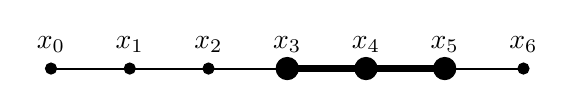
\begin{tikzpicture}[scale=1.0]
  \node at (0.5,9.3) {$x_0$};
  \node at (1.5,9.3) {$x_1$};
  \node at (2.5,9.3) {$x_2$};
  \node at (3.5,9.3) {$x_3$};
  \node at (4.5,9.3) {$x_4$};
  \node at (5.5,9.3) {$x_5$};
  \node at (6.5,9.3) {$x_6$};
  \draw[line width=0.7pt] (0.5,9.0) -- (6.5,9.0);
  \filldraw (0.5,9.0) circle (2.0pt);
  \filldraw (1.5,9.0) circle (2.0pt);
  \filldraw (2.5,9.0) circle (2.0pt);
  \filldraw (3.5,9.0) circle (4.0pt);
  \filldraw (4.5,9.0) circle (4.0pt);
  \filldraw (5.5,9.0) circle (4.0pt);
  \filldraw (6.5,9.0) circle (2.0pt);
  \draw[line width=2.5pt] (3.5,9.0) -- (5.5,9.0);
\end{tikzpicture}


\caption{\texttt{reaction.c} uses discretization \eqref{eq:nl:drfdscheme} at each interior node of the grid.  This corresponds to a three-point stencil, as shown.}
\label{fig:stencilreaction}
\end{figure}

We take the unknowns, or the corresponding grid nodes, to be the vertices of a graph $G=G(J)$, as shown in the top of Figure \ref{fig:fdcolorreaction}.  Graph $G$ has an edge between two vertices if the corresponding unknowns both appear in at least one equation, i.e.~in one instance of equation \eqref{eq:nl:drfdscheme} in this case.

\begin{figure}
\begin{tikzpicture}[scale=1.0]
\node at (-2.25,8.0) {colored graph $G(J)$:};
  \node at (0.5,8.4) {$0$};
  \node at (1.5,8.4) {$1$};
  \node at (2.5,8.4) {$2$};
  \node at (3.5,8.4) {$0$};
  \node at (4.5,8.4) {$1$};
  \node at (5.5,8.4) {$2$};
  \node at (6.5,8.4) {$0$};
  \draw (0.5,8.0) circle (4.0pt);
  \draw[line width=0.6pt] (0.65,8.0) -- (1.35,8.0);
  \draw (1.5,8.0) circle (4.0pt);
  \draw[line width=0.6pt] (1.65,8.0) -- (2.35,8.0);
  \draw (2.5,8.0) circle (4.0pt);
  \draw[line width=0.6pt] (2.65,8.0) -- (3.35,8.0);
  \draw (3.5,8.0) circle (4.0pt);
  \draw[line width=0.6pt] (3.65,8.0) -- (4.35,8.0);
  \draw (4.5,8.0) circle (4.0pt);
  \draw[line width=0.6pt] (4.65,8.0) -- (5.35,8.0);
  \draw (5.5,8.0) circle (4.0pt);
  \draw[line width=0.6pt] (5.65,8.0) -- (6.35,8.0);
  \draw (6.5,8.0) circle (4.0pt);
  \draw[line width=0.75pt] (0.6,7.9) .. controls (1.4,7.5) and (1.6,7.5) .. (2.4,7.9);
  \draw[line width=0.75pt] (1.6,7.9) .. controls (2.4,7.5) and (2.6,7.5) .. (3.4,7.9);
  \draw[line width=0.75pt] (2.6,7.9) .. controls (3.4,7.5) and (3.6,7.5) .. (4.4,7.9);
  \draw[line width=0.75pt] (3.6,7.9) .. controls (4.4,7.5) and (4.6,7.5) .. (5.4,7.9);
  \draw[line width=0.75pt] (4.6,7.9) .. controls (5.4,7.5) and (5.6,7.5) .. (6.4,7.9);
\node at (-2.4,6.9) {colored columns of $J$:};
  %\draw[xstep=1.0,ystep=1.0,black,thin] (0.0,0.0) grid (7.0,7.0);
  \node at (0.5,7.0) {$0$};
  \node at (0.5,6.2) {$0$};
  \node at (1.5,7.0) {$1$};
  \node at (1.5,6.2) {$1$};
  \node at (1.5,5.4) {$1$};
  \node at (2.5,6.2) {$2$};
  \node at (2.5,5.4) {$2$};
  \node at (2.5,4.6) {$2$};
  \node at (3.5,5.4) {$0$};
  \node at (3.5,4.6) {$0$};
  \node at (3.5,3.8) {$0$};
  \node at (4.5,4.6) {$1$};
  \node at (4.5,3.8) {$1$};
  \node at (4.5,3.0) {$1$};
  \node at (5.5,3.8) {$2$};
  \node at (5.5,3.0) {$2$};
  \node at (5.5,2.2) {$2$};
  \node at (6.5,3.0) {$0$};
  \node at (6.5,2.2) {$0$};
\end{tikzpicture}


\caption{Graph $G(J)$ is built from the stencil and the grid, with an edge for every pair of unknowns that appears in an equation in system \eqref{eq:nl:equation}.  Coloring this graph---$c=3$ colors suffice in this case---also assigns colors to the columns of $J$.}
\label{fig:fdcolorreaction}
\end{figure}

Now suppose we color the vertices so that any two vertices which share an edge have distinct colors.  The coloring in the Figure uses $c=3$ colors.  In the case of this simple graph, $c=3$ is the minimum number needed, so that in this case $\chi(G)=c$ where $\chi(G)$ is the \emph{chromatic number} of $G$ \citep{ChartrandLesniakZhang2011}.

The case of a structured 2D grid, as used in Chapter \ref{chap:st} with a finite-difference scheme \eqref{poissonsquareFD} for the Poisson equation \eqref{poissonsquare}, further illustrates the coloring idea.  The stencil of the scheme involves five unknowns $u_{i,j+1}, u_{i-1,j}, u_{i,j}, u_{i+1,j}, u_{i,j-1}$ (Figure \ref{fig:unitsquaregridstencil}).  Therefore the graph $G(J)$ in this case includes a complete graph on five vertices, a $K_5$ \citep{ChartrandLesniakZhang2011}, as a subgraph at each (generic interior) node in the structured grid, as shown in Figure 4.7.  Clearly $\chi(G(J))\ge 5$.  When \PETSc uses a coloring algorithm then it finds that indeed five colors suffice to color $G(J)$.\sidenote{At least in refined-grid cases using the default incidence-degree-ordering.  Certain coarse grids have lower chromatic number.}  We will be able to verify this behavior when we have a \pSNES-based 2D PDE example to work with, as in the next Chapter.
% for number of colors on graph in fig:colorstencilplane, in refined-grid cases, compare
%   $ ./ex5 -da_refine 4 -log_summary -snes_fd_color | grep SNESFunctionEval
% which gives 19 function evals and
%   $ ./ex5 -da_refine 4 -snes_converged_reason -snes_fd_color
% which gives 3 iterations
% we conclude  19=N(c+1)+1=3(c+1)+1  so c = 5

\begin{figure}
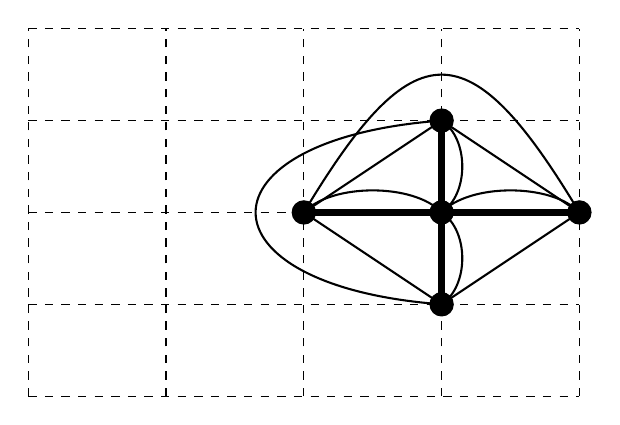
\begin{tikzpicture}[scale=7.0]
% mesh
  \draw[xstep=0.25,ystep=0.166667,black,thin,dashed] (0.0,0.333334) grid (1.0,1.0);
% stencil
  \filldraw (0.50,0.666667) circle (0.6pt);
  \filldraw (0.75,0.666667) circle (0.6pt);
  \filldraw (1.00,0.666667) circle (0.6pt);
  \filldraw (0.75,0.5) circle (0.6pt);
  \filldraw (0.75,0.833333) circle (0.6pt);
% subgraph K_5
  \draw[line width=2.5pt] (0.50,0.666667) -- (1.00,0.666667);
  \draw[line width=2.5pt] (0.75,0.5)  -- (0.75,0.833333);
  \draw[line width=0.75pt] (0.5,0.666667) -- (0.75,0.833333) -- (1.0,0.666667) -- (0.75,0.5) -- cycle;
  \draw[line width=0.75pt] (0.5,0.666667) .. controls (0.55,0.72) and (0.7,0.72) .. (0.75,0.666667);
  \draw[line width=0.75pt] (0.75,0.666667) .. controls (0.8,0.72) and (0.95,0.72) .. (1.0,0.666667);
  \draw[line width=0.75pt] (0.75,0.833333) .. controls (0.8,0.8) and (0.8,0.7) .. (0.75,0.666667);
  \draw[line width=0.75pt] (0.75,0.666667) .. controls (0.8,0.633333) and (0.8,0.533333) .. (0.75,0.5);
  \draw[line width=0.75pt] (0.5,0.666667) .. controls (0.7,1.0) and (0.8,1.0) .. (1.0,0.666667);
  \draw[line width=0.75pt] (0.75,0.833333) .. controls (0.3,0.8) and (0.3,0.533333) .. (0.75,0.5);
\end{tikzpicture}


\caption{For the 2D finite-difference scheme used in Chapter \ref{chap:st}, the graph $G(J)$ has a $K_5$ at every node (thin lines) because the stencil (thick lines) involves five unknowns.}
\label{fig:colorstencilplane}
\end{figure}

Optimally-coloring a graph is a hard problem which \PETSc does not attempt to solve.  \PETSc includes ``incidence-degree ordering'' [\emph{default}] and ``smallest-last ordering'' graph-coloring algorithms which provide $c$-colorings for which $c \le \alpha N^{1/2} \chi(G(J))$ \citep{ColemanMore1983}, for some constant $\alpha>0$, where $N$ is the number of equations in \eqref{eq:nl:equation}.  These algorithms also do well in the informal sense that $c$ is close to $\chi(G(J))$ for a large selection of test matrices \citep{ColemanMore1983}.  Furthermore, these algorithms run in time proportional to the sum of squares of the number of nonzeros in each rows of $J$.  Thus we get a reasonably-good coloring not just in polynomial time in $N$, but in substantially-less time than $O(N^2)$ and often in $O(N)$ time for problems coming from discretized PDEs.\sidenote{Recall we are trying to improve on the existing $O(N^2)$ cost of the \texttt{-snes\_fd} method.}

The graph coloring also implies a coloring of the columns of $J$, as shown in Figure \ref{fig:fdcolorreaction}.  (Each row has distinct colors, which is one way to describe our purpose here.)  The first step in modifying the finite-difference formulas is to generate vectors $\bv_0, \bv_1, \dots, \bv_{c-1} \in \RR^N$ by the rule that $\bv_k$ has a $1$ in entry $j$ if $k$ is the color of unknown $j$, and is otherwise zero.  In the $c=3$ case shown in Figure \ref{fig:fdcolorreaction},
\begin{equation}
\bv_0 = \begin{bmatrix} 1 \\ 0 \\ 0 \\ 1 \\ 0 \\ 0 \\ 1 \end{bmatrix}, \qquad
\bv_1 = \begin{bmatrix} 0 \\ 1 \\ 0 \\ 0 \\ 1 \\ 0 \\ 0 \end{bmatrix}, \qquad
\bv_2 = \begin{bmatrix} 0 \\ 0 \\ 1 \\ 0 \\ 0 \\ 1 \\ 0 \end{bmatrix}.
 \label{eq:nl:coloringvecs}
\end{equation}
We define a function which maps from node (unknown) index $j$ to color $k$,
\begin{equation}
k = k(j),  \label{eq:nl:colorfunc}
\end{equation}
and $(\bv_k)_j = \delta_{k,k(j)}$.  Note $k(j) = j\mod 3$\, in this case.

Then we replace \eqref{eq:nl:fdjac} with
\begin{equation}
J_{ij} = \frac{\partial F_i}{\partial x_j} \approx \frac{F_i(\bx+\delta \bv_{k(j)}) - F_i(\bx)}{\delta}.  \label{eq:nl:fdcolorjac}
\end{equation}
The right sides of \eqref{eq:nl:fdjac} and \eqref{eq:nl:fdcolorjac} compute exactly the same entries $J_{ij}$, but \eqref{eq:nl:fdcolorjac} requires far fewer evaluations of $\bF$.  In particular, all columns of $J$ with color $k$ are computed by \eqref{eq:nl:fdcolorjac} just using the \emph{smallest} $j$ for which $k(j)=k$.  Thus, given a $c$-coloring of $G(J)$ there are exactly $c$ evaluations $\bF(\bx+\delta \bv_{k(j)})$, plus one more for $\bF(\bx)$, to fill $J$ using \eqref{eq:nl:fdcolorjac}.

The news is good when we actually try it.  The result is almost as fast in this 1D PDE case as using the analytical Jacobian:
\begin{cline}
$ timer ./reaction -snes_converged_reason -da_refine 10 -snes_fd_color
Nonlinear solve converged due to CONVERGED_FNORM_RELATIVE iterations 3
on 8193 point grid:  |u-u_exact|_inf/|u|_inf = 1.75633e-10
real 0.06
\end{cline}
%$
Compare the run on page \pageref{etc:nl:bestreaction}.

Counting the number of function evaluations in the various cases is a good idea, and there is no need to alter \texttt{reaction.c} to do so: use \texttt{-log\_summary} and look at the output.\sidenote{Do not add print statements!}  Because we want the ``\texttt{SNESFunctionEval}'' lines, \texttt{grep} extracts the count for the runs above:
\begin{cline}
$ ./reaction -da_refine 10 -snes_fd -snes_max_funcs 100000 -log_summary | grep SNESFunctionEval
SNESFunctionEval   24586 1.0 3.3170e+00 1.0 ...
$ ./reaction -da_refine 10 -snes_fd_color -log_summary | grep SNESFunctionEval
SNESFunctionEval      13 1.0 4.7762e-03 1.0 ...
$./reaction -da_refine 10 -log_summary | grep SNESFunctionEval
SNESFunctionEval       4 1.0 9.3341e-04 1.0 ...
\end{cline}
%$
The number of $\bF$ evaluations was 24586, 13, and 4, respectively.


\section{Jacobian-free Newton-Krylov (JFNK)} \label{sec:JFNK}

Besides the finite-difference Jacobian approach above, using equation \eqref{eq:nl:fdjac} or \eqref{eq:nl:fdcolorjac} to compute the entries of the matrix, there is another approach which requires no assembled Jacobian matrix at all.  It approximates matrix-vector products with the Jacobian matrix by a finite difference formula, and uses a Krylov-type method to solve \eqref{eq:nl:newton:eq} from a space
\begin{equation}
    \mathcal{K} = \operatorname{span}\{\br,J\br,J^2\br,\dots,J^{m-1}\br\}. \label{eq:nl:krylovagain}
\end{equation}
Here $J=J_{\bF}(\bx_k)$ is the Jacobian at iterate $k$ and $\br$ is a (linear) residual in equation \eqref{eq:nl:newton:eq}.

It goes by the name ``Jacobian-free Newton-Krylov'' \citep{KnollKeyes2004} or just ``JFNK''.  To give more detail, suppose we use initial estimate $0$ for the solution to \eqref{eq:nl:newton:eq}.  The residual is $\br = - \bF(\bx) - J 0 = - \bF(\bx)$.  To compute $J\br$, $J^2\br=J(J\br)$, \dots in \eqref{eq:nl:krylovagain}, recall definition \eqref{eq:nl:expandF} of the derivative of $\bF$.  It implies that if $\bv$ is any vector then
\begin{equation}
J \bv \approx \frac{\bF(\bx+\delta \bv) - \bF(\bx)}{\delta} \label{eq:nl:JFNKbasic}
\end{equation}
for small $\delta \ne 0$.  Approximating the Jacobian-vector product by \eqref{eq:nl:JFNKbasic} avoids evaluation of any entries of $J$.

Computing $\br = - \bF(\bx)$, to get the Krylov method started, requires evaluating $\bF$.  Then each successive vector in basis \eqref{eq:nl:krylovagain} requires an additional evaluation of $\bF$, namely
\begin{equation}
J^{\ell} \br \approx \frac{\bF(\bx+\delta J^{\ell-1}\br) - \bF(\bx)}{\delta} \label{eq:nl:JFNKiteration}
\end{equation}
for $\ell=1,\dots,m$.  Equation \eqref{eq:nl:JFNKiteration}, the central calculation in JFNK, uses $m$ evaluations of $\bF$ to compute the whole Krylov basis \eqref{eq:nl:krylovagain}.  By contrast, use of finite difference formula \eqref{eq:nl:fdjac} to compute a generic $N\times N$ Jacobian $J$ requires $N$ evaluations of $\bF$.  Thus JFNK can be efficient if \eqref{eq:nl:newton:eq} is solved to desired tolerance in $m\ll N$ Krylov iterations.

However, there are a few basic points to consider.  First, once you have a matrix you can do many things, such as incomplete matrix factorizations, other than computing a matrix-vector product or a Krylov basis, so giving up on matrices may be premature.  Second, and related, we may need to precondition linear equation \eqref{eq:nl:newton:eq}, in which case we want the Krylov space for the linear operator $M^{-1}J$, not for $J$ itself.  Also, in cases such as structured-grid PDE schemes where it can be applied, we have seen that coloring greatly reduces the cost of using \eqref{eq:nl:fdjac} to assemble $J$.  JFNK is a good strategy to the extent that it actually \emph{works}, and to the extent it beats the competition.

Note JFNK is implemented in \PETSc and invoked by option \texttt{-snes\_mf}, where ``\texttt{mf}'' in stands for ``matrix-free.''\sidenote{The \PETSc API provides functions for even more flexibility and generality than are available at the command line with options \texttt{-snes\_mf}, \texttt{-snes\_fd}, \texttt{-snes\_fd\_color}, and so on.}  We shall see below, in the important and even essential preconditioned case, that there may be a matrix involved in JFNK anyway.  The method never involves fully-assembling the Jacobian matrix itself, however, and thus the ``Jacobian-free'' label is justified.

The issues above can be pursued in more detail on a concrete example, so let us give it a try on a very coarse grid in the 1D diffusion-reaction PDE example \texttt{reaction.c}:
\begin{cline}
$ ./reaction -snes_converged_reason -snes_mf
Nonlinear solve converged due to CONVERGED_FNORM_RELATIVE iterations 3
on 9 point grid:  |u-u_exact|_inf/|u|_inf = 0.000188753
\end{cline}
%$
So far so good.

Any enthusiasm is rather damped when we try refined grids.  Noting $J$ is symmetric in this case,\sidenote{Well \dots nearly so.  See exercise 4.\ref{exer:nl:symmetrizeJ}.} we try the CG method (Chapter \ref{chap:ls}) and ask \PETSc for both the number of Newton and Krylov iterations.  On 500 and 1000 point grids the performance is poor in the sense that too many ``inner'' Krylov iterations are needed:
\begin{cline}
$ ./reaction -snes_converged_reason -snes_mf -ksp_converged_reason -ksp_type cg -da_refine 6
  Linear solve converged due to CONVERGED_RTOL iterations 511
  Linear solve converged due to CONVERGED_RTOL iterations 504
  Linear solve converged due to CONVERGED_RTOL iterations 508
Nonlinear solve converged due to CONVERGED_FNORM_RELATIVE iterations 3
on 513 point grid:  |u-u_exact|_inf/|u|_inf = 4.62255e-08
$ ./reaction -snes_converged_reason -snes_mf -ksp_converged_reason -ksp_type cg -da_refine 7
  Linear solve converged due to CONVERGED_RTOL iterations 1023
  Linear solve converged due to CONVERGED_RTOL iterations 1006
  Linear solve converged due to CONVERGED_RTOL iterations 1015
  Linear solve converged due to CONVERGED_RTOL iterations 950
Nonlinear solve converged due to CONVERGED_FNORM_RELATIVE iterations 4
on 1025 point grid:  |u-u_exact|_inf/|u|_inf = 1.15576e-08
\end{cline}
These large iteration counts, which illustrate the well-known doubling of CG iterations with each doubling of dimension, also arose in Chapter \ref{chap:ls} when we looked at unpreconditioned Krylov methods.

Observe that the default GMRES solver is no better; we simply get a linear solve failure:
\begin{cline}
$ ./reaction -snes_converged_reason -snes_mf -ksp_converged_reason -da_refine 7
  Linear solve did not converge due to DIVERGED_ITS iterations 10000
Nonlinear solve did not converge due to DIVERGED_LINEAR_SOLVE iterations 0
on 1025 point grid:  |u-u_exact|_inf/|u|_inf = 0.217386
\end{cline}
%$

Here we see an excellent reminder to apply the Krylov solver to a \emph{preconditioned} form of linear equation \eqref{eq:nl:newton:eq}.  In this case left- and right-sided preconditioning, equations \eqref{introleftpre} and \eqref{introrightpre} in Chapter \ref{chap:ls}, are
\begin{align}
(M^{-1} J) \bs &= - M^{-1} \bF(\bx_k), \label{eq:nl:leftpre} \\
(J M^{-1}) (M \bs) &= - \bF(\bx_k), \label{eq:nl:rightpre}
\end{align}
respectively.  Regarding their implementation in the Krylov iteration, in \eqref{eq:nl:leftpre} the action of $M^{-1} J$ on some vector $\bv$ is a straightforward composition of \eqref{eq:nl:JFNKbasic} followed by application of $M^{-1}$.  In right preconditioning \eqref{eq:nl:rightpre} the action of $J M^{-1}$ on $\bv$ is computed by first applying $M^{-1}$ to $\bv$, namely by solving $M \by = \bv$, and then using \eqref{eq:nl:JFNKbasic}:
\begin{equation}
(J M^{-1}) \bv \approx \frac{\bF(\bx+\delta \by) - \bF(\bx)}{\delta} \label{eq:nl:JFNKwithrightpre}
\end{equation}

Also recall that preconditioning matrices $M$ and $M^{-1}$ are usually never assembled.  Even if an assembled preconditioner-material matrix $P$ is present, $M$ is generally constructed nontrivially from $P$.  For example, if we supply some assembled matrix $P$ as the preconditioner material, but we ask for ILU($0$) preconditioning, then $M$ is actually the product of the ILU($0$) factors of $P$, not $P$ itself.


\section{Jacobian cases} \label{sec:jacobiancases}

\def\checkmark{\tikz\fill[scale=0.4](0,.35) -- (.25,0) -- (.7,.8) -- (.25,.15) -- cycle;}
\def\bigcheckmark{\tikz\fill[scale=0.6](0,.35) -- (.25,0) -- (.7,.8) -- (.25,.15) -- cycle;}

At this point we risk overwhelming the reader with options, so we pause to review the possibilities before testing them on the \texttt{reaction.c} problem.

Table \ref{tab:snesjacobianoptions:needed} summarizes options relating to residual and Jacobian call-backs in \pSNES-using codes.  If no Jacobian or approximate Jacobian routine is provided in the user-written code then only finite-difference evaluation of an assembled Jacobian matrix (i.e.~\texttt{-snes\_fd} or \texttt{-snes\_fd\_color}) or finite-difference evaluation of the Jacobian-vector product inside the Krylov method (\texttt{-snes\_mf}, i.e.~JFNK) are available.  If a Jacobian routine \emph{is} provided then it is used in the Newton iteration (when no alternative option is given).

However, option \texttt{-snes\_mf\_operator}, which we have not mentioned until now, tells the \pSNES to only use the provided Jacobian when preconditioning the JFNK Jacobian-vector product.  This last option may give quadratic convergence even if the provided Jacobian is inexact, that is, even if the ``material'' $P$ which is used to build $M$ in formulas \eqref{eq:nl:leftpre}--\eqref{eq:nl:JFNKwithrightpre} is only an approximation of the Jacobian $J$.

\begin{table}
\begin{tabular}{lllll}
 &\underline{\small no option}\hspace{0.0in} & \underline{\small\hspace{-0.05in}$\begin{array}{ll} \text{\texttt{-snes\_fd}} \\ \text{\texttt{-snes\_fd\_color}}\end{array}$} & \underline{\small \texttt{-snes\_mf}} & \underline{\small \texttt{-snes\_mf\_operator}} \\
only $\bF$      & error           & $\bigcheckmark$ & $\bigcheckmark$ & error \\
$\bF$ and $P$   & $\checkmark$ & $\checkmark$    & $\checkmark$    & $\bigcheckmark$ \\
$\bF$ and $J$   & $\bigcheckmark$ & $\checkmark$    & $\checkmark$    & $\checkmark$
\end{tabular}
\caption{Jacobian options when using \pSNES.  The row labels describe which mathematical objects have been provided through user-implemented code.  Symbol ``$P$'' denotes an approximate Jacobian while ``$J$'' denotes the actual Jacobian.  A larger check mark shows recommended usage.} \label{tab:snesjacobianoptions:needed}
\end{table}

From the code side, at a minimum a method for $\bF$ must be implemented in all cases, as there is no other way for \PETSc to know what equations you are solving.\sidenote{Except in the case where the residual function $\bF$ itself represents a derivative (gradient) of an objective function.  See Chapter \ref{chap:of}.}   There are two ways of providing $\bF$:  If the problem is based on a structured grid, as in \texttt{reaction.c} above, use \texttt{DMDASNESSetFunctionLocal()}.  In general, use \texttt{SNESSetFunction()}.  If only $\bF$ is provided, do not create or preallocate a \pMat for the Jacobian, as this is done internally by the \pSNES for \texttt{-snes\_fd} and \texttt{-snes\_fd\_color} runs, while no assembled Jacobian \pMat exists for \texttt{-snes\_mf} runs.

If an exact ($J$) or approximate ($P$) Jacobian function is implemented then there are two cases:
\begin{quote}
  \renewcommand{\labelenumi}{(\roman{enumi})}
  \begin{enumerate}
  \item On a structured grid, provide the function (e.g.~``\texttt{FormJacobianLocal()}'') using \texttt{DMDASNESSetJacobianLocal()}.  In this case the \pMat holding the Jacobian is internal, and so it is not created or preallocated by the user.
  \item In a general, first declare a \pMat variable, say ``\texttt{J}'', and then call \texttt{MatCreate()}, \texttt{MatSetSizes()}, and \texttt{MatSetFromOptions()} on it.  Then call either \texttt{MatSetUp()} or \texttt{MatXAIJPreallocate()} on \texttt{J}, to allocate space for the assembled Jacobian matrix.  Then provide the call-back code for function $J$ or $P$ (e.g.~``\texttt{FormJacobian()}'') and the \pMat \texttt{J} for both \pMat arguments through \texttt{SNESSetJacobian()}.
  \end{enumerate}
\end{quote}
In either case (i) or (ii), the user's Jacobian code only needs to set values in the second ``preconditioner'' \pMat argument.  (This assumes in (ii) that \texttt{J} is provided for both \pMat arguments of \texttt{SNESSetJacobian()}, as described.)  The code should, however, \emph{assemble} both \pMat arguments.

As practical advice for the debugging stage, you know you have correctly- and fully-implemented the Jacobian, and you have found an adequate initial iterate, if all four options (columns) in Table \ref{tab:snesjacobianoptions:needed} work and each gives apparent quadratic convergence when looking at the residual norm decay shown by \texttt{-snes\_monitor}.  As the reader may check, this is the situation for the last two codes \texttt{ecjacobian.c} and \texttt{reaction.c}.

Another way to compare the options, especially in a structured PDE case where option \texttt{-snes\_fd\_color} might be effective, is shown in Table \ref{tab:snesjacobianoptions:evals}.  This Table supposes, rather unrealistically, that the number $q$ of Newton iterations is independent of the option.  For the last column it also assumes, again unrealistically, that the number of Krylov iterations is the same at each Newton iteration (in JFNK).  The Table two simple points:\begin{itemize}
\item Improved performance with \texttt{-snes\_fd\_color} comes from having a $c$-coloring where $c \ll N$.
\item Improved performance with \texttt{-snes\_mf\_operator} comes from reducing the number $m$ of Krylov iterations.  We know from Chapter \ref{chap:ls} that this is primarily an issue of choosing the right preconditioner so that $m_2 \ll m_1$.
\end{itemize}

\begin{table}
\begin{tabular}{lccc}
 &\underline{no option}
                       & \small\underline{$\begin{array}{ll} \text{\texttt{-snes\_fd}} \\ \text{\texttt{-snes\_fd\_color}} \end{array}$}
                                    & \small\underline{$\begin{array}{ll} \text{\texttt{-snes\_mf}} \\ \text{\texttt{-snes\_mf\_operator}} \end{array}$} \vspace{0.2in} \\
residual $\bF$        & $q+1$ & $\begin{array}{cc} q(N+1)+1 \\ q(c+1)+1 \end{array}$ & $\begin{array}{cc} q m_1 \\ q m_2 \end{array}$ \vspace{0.1in} \\
Jacobian $J$ or $P$    & $q$ & $\begin{array}{cc} 0 \\ 0 \end{array}$ & $\begin{array}{cc} 0 \\ q \end{array}$
\end{tabular}
\caption{Jacobian options compared by number of residual and Jacobian evaluations.  Here $q$ is the number of Newton iterations, $N$ is the dimension of the problem, $c$ is the number of colors on $G(J)$, $m_1$ is the dimension of the Krylov space for $J$, and $m_2$ is the Krylov space dimension for the preconditioned operator $M^{-1}J$.} \label{tab:snesjacobianoptions:evals}
\end{table}


\section{Testing JFNK with preconditioning} \label{sec:testsnesmfoperator}

We now do refined-grid runs of \texttt{reaction.c} to show the \texttt{-snes\_mf\_operator} option in action.  We have already seen that the \texttt{-snes\_fd\_color} option is effective for reducing evaluations of $\bF$ if a Jacobian is not implemented, but in the same case the un-preconditioned JFNK method \texttt{-snes\_mf} has serious difficulties as it requires unreasonable numbers of Krylov iterations and function evaluations.  Now we can show that \texttt{-snes\_mf\_operator} using only a rough approximation of the Jacobian as a preconditioner gives good performance.

Specifically, suppose we modify this line in \texttt{reaction.c} (Code \ref{code:reactionI}),
\begin{code}
    col[1] = i;    v[1] = 2.0 - h*h * dRdu;
\end{code}
to remove ``\texttt{- h*h * dRdu}'', corresponding to the nonlinear term $\rho \sqrt{u}$ in \eqref{eq:nl:drsqrt}, to obtain
\begin{code}
    col[1] = i;    v[1] = 2.0;
\end{code}
This change, which we call a ``\texttt{J->P}'' below, keeps the tridiagonal sparsity pattern of the Jacobian.  Furthermore it preserves many characteristics of the spectrum of the linearizations of the operator in \eqref{eq:nl:drsqrt} by keeping the highest-order term $u''$.

With this change, convergence is slowed for no option, that is, when we try to use the new approximate Jacobian as though it were exact.  Specifically, on a coarse grid the number of iterations goes from 4 to 15, and the residual norms suggest that convergence is no longer quadratic:
\begin{cline}
$ ./reaction -da_refine 4 -snes_monitor    # before change
  0 SNES Function norm 1.671129624018e-02 
  1 SNES Function norm 3.609252641302e-04 
  2 SNES Function norm 4.167490508951e-07 
  3 SNES Function norm 4.935230509260e-13 
on 129 point grid:  |u-u_exact|_inf/|u|_inf = 7.39662e-07
$ ./reaction -da_refine 4 -snes_monitor    # with J->P change
  0 SNES Function norm 1.671129624018e-02 
  1 SNES Function norm 3.822032062916e-03 
...
 14 SNES Function norm 3.879363487638e-10 
 15 SNES Function norm 1.119521798815e-10 
on 129 point grid:  |u-u_exact|_inf/|u|_inf = 7.38159e-07
\end{cline}
This loss of Newton method performance from a significantly incorrect Jacobian is expected in theory \citep{Kelley2003}.

However, for this modified Jacobian case, \texttt{-snes\_mf\_operator} is now a fast option for higher-resolution grids, fully competitive with the exact Jacobian and finite-difference-by-coloring cases already seen.  Again on a $8000$ point grid, using the approximate Jacobian ``as is'' causes too many Newton iterations and less-than-quadratic convergence:
\begin{cline}
$ timer ./reaction -snes_converged_reason -da_refine 10    # with J->P change
Nonlinear solve converged due to CONVERGED_FNORM_RELATIVE iterations 15
on 8193 point grid:  |u-u_exact|_inf/|u|_inf = 1.36236e-09
real 0.13
\end{cline}
%$
Now we try \texttt{-snes\_mf\_operator}, which is designed for this approximate-Jacobian situation:
\begin{cline}
$ timer ./reaction -snes_converged_reason -da_refine 10 -snes_mf_operator  # with J->P change
Nonlinear solve converged due to CONVERGED_FNORM_RELATIVE iterations 4
on 8193 point grid:  |u-u_exact|_inf/|u|_inf = 1.80588e-10
real 0.05
\end{cline}
%$
The number of iterations and the time are significantly reduced, and both are comparable to the exact Jacobian case (page \pageref{etc:nl:bestreaction}).

One might give the following summary advice on \pSNES usage:

\begin{quote}
Before implementing a Jacobian, try finite-difference evaluation \texttt{-snes\_fd} first, including a look at whether coloring (option \texttt{-snes\_fd\_color}) applies to your case.  As a general rule, it can be applied and it is often effective on a structured grid, but on an unstructured grid (Chapters \ref{chap:un} and \ref{chap:dp}) the coloring method requires additional work.  Note JFNK with no preconditioning (option \texttt{-snes\_mf}) is rarely effective, though easy to try.  Now consider implementing the exact Jacobian $J$.  If that seems like too much work or is too error-prone, consider a simpler approximate Jacobian $P$ used with option \texttt{-snes\_mf\_operator}.  In PDE cases, in particular, $P$ might only capture the highest-order derivatives in $J$.  To test convergence with $P$, compare ``no option'' runs which use $P$ as though it were $J$, but wherein less-than-quadratic convergence is expected, and \texttt{-snes\_mf\_operator} runs where quadratic convergence should be recovered.
\end{quote}


\section{Line search Newton methods} \label{sec:linesearch}

Once the Newton step $\bs_k$ solving equation \eqref{eq:nl:newton:eq} is computed, the new iterate $\bx_{k+1} = \bx_k + \bs_k$ from \eqref{eq:nl:newton:update} may not be what we want.  For example, the residual norm $\|\bF(\bx_k + \bs_k)\|$ may exceed $\|\bF(\bx_{k})\|$, suggesting that no progress is being made in solving \eqref{eq:nl:equation}.  Improving this situation is the problem of \emph{globalizing} the convergence of the Newton iteration, so that the iterates $\bx_k$ are more likely to head toward the sometimes-small region of quadratic convergence around the solution to \eqref{eq:nl:equation}.

The \emph{line search} globalization technique \citep{DennisSchnabel1983} is to replace \eqref{eq:nl:newton:update} with
\begin{equation}
\bx_{k+1} = \bx_k + \lambda_k \bs_k.  \label{eq:nl:linesearchupdate}
\end{equation}
That is, we accept $\bs_k$ as a search direction for solving \eqref{eq:nl:newton:eq}, but we may use an actual step of less ($\lambda_k < 1$), or sometimes more ($\lambda_k > 1$), than in \eqref{eq:nl:newton:update}.  The question, of course, is how to choose $\lambda_k$.

As we are solving a system of nonlinear equations \eqref{eq:nl:equation}, there is no pre-existing sense of ``better'' or ``worse'' approximations, as there is in an optimization context.  But we may introduce a particular \emph{merit function} \citep{NocedalWright2006} to provide such a sense, namely
\begin{equation}
\phi(\bx) = \frac{1}{2} \|\bF(\bx)\|_2^2.  \label{eq:nl:linesearchmeritfunction}
\end{equation}
This merit function is used in all \pSNES line searches, unless an objective function is provided to the \pSNES (next Chapter).

To determine $\lambda_k$ one could perhaps solve the one-dimensional optimization problem
\begin{equation}
\min_{0<\lambda} \phi(\bx_k + \lambda \bs_k),  \label{eq:nl:linesearchperhapsopt}
\end{equation}
thereby making the residual 2-norm as small as possible along the search direction.  However, solving this optimization problem accurately is rarely-justified because we are merely using the solution to compute the next Newton iterate; we hope the Newton iteration itself, with $\lambda=1$, generates rapid convergence.

A practical line-search tries candidate values of $\lambda=\lambda_k$, testing them for whether they reduce $\phi(\bx_k + \lambda \bs_k)$.  The initial try is usually $\lambda=1$.  A \emph{sufficient  decrease} condition with parameter $\alpha\in(0,1)$ is to require
\begin{equation}
\phi(\bx_k + \lambda \bs_k) \le \phi(\bx_k) + \alpha \lambda\, \bs_k^\top \grad \phi(\bx_k).  \label{eq:nl:linesearchsuffdecrease}
\end{equation}
The \PETSc default for $\alpha$ is $10^{-4}$, corresponding to an easy-to-satisfy reduction criterion, and the Newton iteration is stopped with an error if such a decrease cannot be found.

The quantity $\bs_k^\top \grad \phi(\bx_k)$ in \eqref{eq:nl:linesearchsuffdecrease} is an initial slope of $\phi(\bx)$ as we move in the search direction---it is the directional derivative in the direction $\bs_k$.  In fact, for merit function \eqref{eq:nl:linesearchmeritfunction} it is always negative, as we see by using \eqref{eq:nl:newton:eq}:
\begin{align}
\bs_k^\top \grad \phi(\bx_k) &= \bs_k^\top J_{\bF}(\bx_k)^\top \bF(\bx_k) = \left(J_{\bF}(\bx_k) \bs_k\right)^\top \bF(\bx_k) \label{eq:nl:linesearchinitslope} \\
  &= - \|\bF(\bx_k)\|_2^2. \notag
\end{align}
Thus $\bs_k$ is a descent direction for merit function \eqref{eq:nl:linesearchmeritfunction}.  Also notice that sufficient decrease condition \eqref{eq:nl:linesearchsuffdecrease} can be evaluated using only residual evaluations $\bF(\bx_k)$ and $\bF(\bx_k + \lambda \bs_k)$.

Merit function \eqref{eq:nl:linesearchmeritfunction} has another nice property.  Though $\phi(\bx)$ may have local minima $\bx'$ other than solutions $\bx^*$ to \eqref{eq:nl:equation}, the Jacobian must also be singular at such locations.  In fact,
\begin{equation}
0 = \grad \phi (\bx') = J_{\bF}(\bx')^\top \bF(\bx'),
\end{equation}
so $J_{\bF}(\bx')^\top$ has a nonzero null-space if $\bF(\bx')\ne 0$.  Thus, for example, no non-solution local minima arise in a region where there is a finite bound on the condition number of the Jacobian.

The line search options available in \PETSc are summarized in Table \ref{tab:nl:linesearchoptions}.  The Table has only minimal information, so for more details see \citep[Chapter 6]{DennisSchnabel1983} and the \PETSc source code itself.

\begin{table}
\begin{tabular}{ll}
\underline{Name} & \underline{Summary} \vspace{0.05in} \\ \vspace{0.1in}
\texttt{basic} & No line search.  Use full Newton step $\lambda_k=1$ in \eqref{eq:nl:linesearchupdate}. \\ \vspace{0.1in}
\texttt{bt} [\emph{default}] & \begin{minipage}[t]{0.8\textwidth}
Polynomial-fit back-tracking \citep[section 6.3.2]{DennisSchnabel1983}.  A quadratic or cubic [\emph{default}] polynomial is built up as a model for \mbox{$\phi(\bx_k+\lambda \bs_k)$}, though initially the model is always quadratic.  Successive values $\lambda$ are required to decrease.
\end{minipage} \\ \vspace{0.1in}
\texttt{cp} & \begin{minipage}[t]{0.83\textwidth}
Assumes $\bF$ is the gradient of an unknown objective function, i.e.~\mbox{$\bF=\grad g$}.  A critical point of $g$ is then found along the search direction by the secant method.
\end{minipage} \\ \vspace{0.1in}
\texttt{l2} & \begin{minipage}[t]{0.83\textwidth}
Secant-line minimization along the search direction, starting with testing \mbox{$\lambda=1/2$} and \mbox{$\lambda=1$}. Repeated a fixed number of times.
\end{minipage}
\end{tabular}
\caption{Line search methods (types) for \pSNES.  Use \texttt{-snes\_linesearch\_type X} to choose one.  Only types \texttt{bt} and \texttt{l2} use an objective function, supposing it is provided by a call to \texttt{SNESSetObjective()}.  Sufficient decrease \eqref{eq:nl:linesearchsuffdecrease} is only tested in type \texttt{bt}.} \label{tab:nl:linesearchoptions}
\end{table}

One chooses line search type \texttt{X} by option \texttt{-snes\_linesearch\_type X}.  Option \texttt{-snes\_linesearch\_monitor} shows runtime diagnostics.  Parameter $\alpha$ in sufficient decrease condition \eqref{eq:nl:linesearchsuffdecrease} can be set, in the rare case where this is needed, by \texttt{-snes\_linesearch\_alpha}.  The initial value for $\lambda_k$ can be set by \texttt{-snes\_linesearch\_damping}, with default of $1$.  Option \texttt{-snes\_linesearch\_max\_it} sets the maximum number of line search tries for type \texttt{bt}, but for types \texttt{l2} and \texttt{cp} it sets the fixed number of repetitions of the secant line calculation.  As usual, find all such options by
\begin{cline}
$ ./reaction -help | grep snes_linesearch
\end{cline}
%$

We have actually only been describing one type of \pSNES solver in the last section, namely the line-search \pSNES type chosen by \texttt{-snes\_type newtonls}.  There are also trust region methods \citep{NocedalWright2006} (\texttt{-snes\_type newtontr}) as well as variations on nonlinear preconditioning, but they are not used in this book.  See the \PETSc User's Manual \citep{petsc-user-ref}.

%FIXME: from petsc-users by Matt:  What happens if you use LU? When debugging a nonlinear solver always use a direct solver for the linear solver (and make sure the direct solver actually worked).

\section{Exercises}

\renewcommand{\labelenumi}{\arabic{chapter}.\arabic{enumi}\quad}
\renewcommand{\labelenumii}{(\alph{enumii})}
\begin{enumerate}
\item One needs to \emph{see} quadratic convergence to believe it.  Observe that for $x_k$ in both parts (b) and (c) below, the \emph{number of correct digits in $x_k$ doubles} at each iteration.
    \begin{enumerate}
    \item The sequence $x_k = 1-2^{-n}$ converges to $x^*=1$, but linearly instead of quadratically.  Find $k$ so that $|e_k| < 10^{-16}$.
    \item The sequence $x_k = 1-2^{(-2^n)}$ converges quadratically to $x^*=1$.  Find $k$ so that $|e_k| < 10^{-16}$.  Find the smallest $K$ so that $|e_{k+1}| \le K |e_k|^2$ for all $k$.
    \item Let $F(x) = \cos(x-1) - \exp(1-x)$ and $x_0=0.5$.  Using either \PETSc or a quick-and-dirty numerical tool, compute Newton iterates $x_k$ for $k=1,\dots,6$.  Estimate $K$ so that $|e_{k+1}| \le K |e_k|^2$ for large $k$.
    \end{enumerate}

\item Make a tiny modification to \texttt{ecjacobian.c} to set the initial vector to $\bx_0 = [10\,\, 10]^\top$.  Rerun it with option \texttt{-snes\_monitor} and note it does not converge to a solution.  Why does the \pSNES stop?  Add one runtime option so that it converges, thereby producing the data shown in Figure \ref{fig:newtonconvdelayed}.

\item \label{exer:nl:snestestdisplay}  Run and interpret the result:
\begin{cline}
$ ./ecjacobian -snes_type test -snes_test_display
\end{cline}
%$

\item  \label{exer:nl:newtonatan}
This exercise shows that the original Newton iteration can diverge or enter a limit cycle, according to the initial iterate $x_0$, while using linesearch gives essentially global convergence.
    \begin{enumerate}
    \item By straightforward modifications of \texttt{expcircle.c}, write a code \texttt{atan.c} which solves nonlinear equation \eqref{eq:nl:equation} with $F(x)=\arctan(x)$ and initial iterate $x_0=2.0$.  Observe that running it \texttt{./atan -snes\_fd -snes\_linesearch\_type basic} causes it to diverge, but the default choice \texttt{-snes\_linesearch\_type bt} gives convergence.
    \item Returning to paper calculation, require the Newton iteration \eqref{eq:nl:newton} to enter a sign-flipping limit cycle, i.e.~so that $x_{k+1} = - x_k$ for all $k$.  Thereby approximate the positive value $x_0$ so that the Newton iteration both makes no progress, and remains bounded, for all $k$.\sidenote{One should solve this problem with Newton's method!}  Sketch the situation.
    \item By modifying $x_0$ in \texttt{atan.c} and using linesearch type \texttt{basic}, confirm that one can make the Newton iteration ``stick'' in this actually-unstable limit cycle for quite a while.  Then confirm that linesearch types \texttt{bt,l2,cp} all get unstuck immediately.
% to solve:  - x = x - arctan(x) (1+x^2)
% octave:
%   G = @(x) 2*x - atan(x) * (1+x^2);
%   J = @(x) 1 - atan(x) * (2*x);
%   x = 1.4;
%   format long g
%   for j = 1:4, x = x - G(x) / J(x), end
% get:
%  x = 1.39174520027073
    \end{enumerate}

\item Option \texttt{-log\_summary} can show whether function evaluations or linear solves are dominating the cost of Newton's method.  By looking at \texttt{-log\_summary} output, compare where the work is done in these runs: \texttt{./reaction}, \texttt{./reaction -snes\_fd}, \texttt{./reaction -snes\_mf}.  Does the comparison change if you add \texttt{-da\_refine 5}?  Explain as much as you can.  (\emph{Hints}: Look at \texttt{SNESSolve} events for the total time spent in the Newton method, which is $\approx$100\% for these cases.  Within that event, event \texttt{SNESLineSearch} is where function and Jacobian evaluations happen, while the linear solve is the \texttt{KSPSolve} event.  Within the \texttt{SNESLineSearch} event, look at \texttt{SNESFunctionEval} and \texttt{SNESJacobianEval} events.)

\item \label{exer:nl:symmetrizeJ}  In Chapter \ref{chap:st} we gave some advice which we have not followed in the current Chapter, namely that one should implement Dirichlet conditions in a manner that preserves the symmetry of the matrix in question, which is the Jacobian here.  Modify \texttt{reaction.c} to preserve symmetry, noting that this requires modifying both the $\bF$ and $J$ evaluation routines.  Does this modification improve performance when using the CG iteration?  Does it change our conclusions about un-preconditioned JFNK?

\item The PDE problem in \texttt{reaction.c} has parameter $\rho$ which can be adjusted via \texttt{PetscOptionsReal()}.  Modify \texttt{reaction.c} to a new code ``\texttt{optreact.c}'' and add an option \texttt{-optr\_rho} to read $\rho$ at runtime.  (The prefix \texttt{optr\_} is added when you call \texttt{PetscOptionsBegin()}.)  By sampling, for what range of positive \texttt{X} does the run
\begin{cline}
$ ./optreact -snes_monitor -da_refine 4 -optr_rho X
\end{cline}
%$
converge?  Explain why this case, with this way of choosing the boundary conditions and initial iterate, in contrast to the next Exercise, is insensitive to the value of the major parameter $\rho$.
% because this option is used in bratu.c below, for simplicity of maintenance, the result optreact.c is NOT saved in c/ch4/solns/

\item \label{exer:nl:bratu} Modify \texttt{reaction.c} to create ``\texttt{bratu.c}'' which solves
\begin{equation}
    - u'' - \lambda e^u = 0 \label{eq:nl:bratuoned}
\end{equation}
% R(u) = lambda e^u increasing
with Dirichlet boundary conditions $u(0)=u(1)=0$.  Make $\lambda$ an option-adjustable real parameter---see the previous Exercise---and use the simplest function which satisfies the boundary conditions as an initial iterate.  Confirm by using a fine grid, and option \texttt{-snes\_converged\_reason} plus other options as needed, that around $\lambda=3.513$ there is a transition to non-convergence of the Newton iteration.  This \emph{critical value} is intrinsic to the nonlinear PDE problem and not a result of a Newton failure \citep{Doedeletal1991}.

\item To the author's knowledge an exact solution of \eqref{eq:nl:bratuoned} cannot be written in elementary functions for $\lambda>0$.  Because we started from \texttt{reaction.c}, writing the code in the last exercise is doable.  However, one should not walk over high wires too often without a net, and having an exact solution to check correctness is such a ``net.''  Fortunately, we can ``manufacture'' \citep{Wesseling2001} an exact solution to a generalized form of \eqref{eq:nl:bratuoned}, namely to equation \eqref{eq:nl:diffusionreaction} in the case where $R(u)=-\lambda e^u$.  For example we can choose $u(x) = \sin(\pi x)$ as the exact solution of \eqref{eq:nl:diffusionreaction}, and then determine $f(x)$ from the equation itself.  Here $u(0)=u(1)=0$ are the boundary conditions; they are satisfied by the exact solution.

The exercise itself: Add options and such a manufactured exact solution to the code \texttt{bratu.c} in the previous Exercise.  The new code will both solve the previous Exercise and be verified using the new exact solution, according to a new boolean member \texttt{manufactured} of \texttt{AppCtx}: when it is false then $f(x)=0$ and the code solves the previous Exercise, but if it is true then we report a numerical error based on the manufactured solution.  Implement option \texttt{-bratu\_manu} to set this boolean.  Observe that $f(x)\ne 0$ does not change the Jacobian.  Confirm that in the manufactured-solution case we have both quadratic convergence of the Newton iteration on a fixed grid \emph{and} $O(h^2)$ convergence of the numerical error under grid refinement.

\item As long as the number of MPI processes does not exceed the number of grid points, \texttt{reaction.c} will solve correctly, though perhaps not efficiently, in parallel.  Confirm this by running
\begin{cline}
$ mpiexec -n N ./reaction -snes_converged_reason -da_refine M
\end{cline}
%$
with a few values of \texttt{N} and \texttt{M}.  However, \texttt{ecjacobian.c} does not run correctly even on two MPI processes.  Modify so that it does.

\end{enumerate}
